
% Archivo: informe3.tex

\documentclass[11pt,a4paper]{article}

% Idioma y tipografías
\usepackage[english]{babel}
\usepackage[T1]{fontenc}
\usepackage[utf8]{inputenc}
\usepackage{lmodern}

% Maquetación y tipografía fina
\usepackage[a4paper,margin=2.5cm]{geometry}
\usepackage{microtype}
\usepackage{setspace}
\onehalfspacing

% Utilidades
\usepackage{csquotes}
\usepackage{graphicx}
\usepackage{xcolor}
\usepackage{booktabs}
\usepackage{siunitx}
\usepackage{amsmath,amssymb}
\usepackage{enumitem}
\usepackage{float}
\setlist{nosep,leftmargin=*,labelsep=0.5em}

% Hipervínculos
\usepackage[hidelinks]{hyperref}
\hypersetup{
    pdftitle={Informe de Aprendizaje Difuso},
    pdfauthor={Juan Diego Gallego Nicolás, Óscar Vera López},
    pdfsubject={Aprendizaje Difuso},
    pdfkeywords={Zona de Vida de Holdridge, Lógica Difusa, Inferencia Difusa}
}

% Bibliografía
\usepackage[
    backend=biber,
    style=ieee,
    sorting=nyt,
    maxbibnames=99
]{biblatex}
\addbibresource{references.bib}

% Subfiguras
\usepackage{subcaption}

% Código (Python)
\usepackage{listings}
\lstset{
	language=Python,
	basicstyle=\ttfamily\small,
	keywordstyle=\color{blue},
	stringstyle=\color{red},
	commentstyle=\color{green!60!black}\itshape,
	numbers=left,
	numberstyle=\tiny,
	stepnumber=1,
	numbersep=5pt,
	showstringspaces=false,
	breaklines=true,
	frame=single,
	captionpos=b
}
% Código JSON
\lstdefinelanguage{JSON}{
    basicstyle=\normalfont\ttfamily,
    numbers=left,
    numberstyle=\tiny,
    stepnumber=1,
    numbersep=8pt,
    showstringspaces=false,
    breaklines=true,
    frame=single,
    literate=
     *{0}{{{\color{blue}0}}}{1}
      {1}{{{\color{blue}1}}}{1}
      {2}{{{\color{blue}2}}}{1}
      {3}{{{\color{blue}3}}}{1}
      {4}{{{\color{blue}4}}}{1}
      {5}{{{\color{blue}5}}}{1}
      {6}{{{\color{blue}6}}}{1}
      {7}{{{\color{blue}7}}}{1}
      {8}{{{\color{blue}8}}}{1}
      {9}{{{\color{blue}9}}}{1}
      {:}{{{\color{red}:}}}{1}
      {,}{{{\color{red},}}}{1}
      {\{}{{{\color{orange}\{}}}{1}
      {\}}{{{\color{orange}\}}}}{1}
      {[}{{{\color{orange}[}}}{1}
      {]}{{{\color{orange}]}}}{1}
      {"}{{{\color{green}"}}}{1}
}


% Comandos útiles

\begin{document}
\begin{titlepage}
    \centering
    % \includegraphics[height=2cm]{logo.png}\par\vspace{1cm} % Descomentar si hay logo
    {\Large Informe Técnico 4}\par\vspace{0.5cm}
    {\huge\bfseries Aprendizaje Difuso\par}\vspace{0.5cm}
    \begin{tabular}{@{}ll@{}}
        Autor 1: & Juan Diego Gallego Nicolás \\
        Contacto 1: & jdiego.gallego@um.es \\
        Autor 2: & Óscar Vera López \\
        Contacto 2: & oscar.veral@um.es \\
        Profesor: & Maria del Carmen Garrido Carrera \\
        Asignatura: & Conocimiento y Razonamiento Aproximado \\
    \end{tabular}
    % Include umu logo
    \vfill
    
\includegraphics[height=8cm]{images/SelloUMU-negativo.png}\par\vspace{1cm}
    \vfill
    {\large \today}\par
\end{titlepage}

\pagenumbering{roman}
\clearpage

\tableofcontents
\clearpage
\pagenumbering{arabic}

\section{Ejercicio 1}

Supongamos la siguiente red bayesiana proporciocionada por un experto de una empresa energética:
\begin{figure}[H]
    \centering
    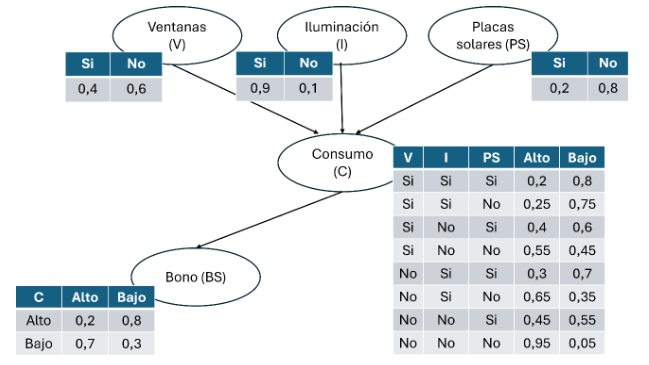
\includegraphics[width=0.6\textwidth]{images/red_bayesiana.png}
    \caption{Red bayesiana proporcionada por el experto.}
    \label{fig:red_bayesiana}
\end{figure}
En la red aparecen 5 variables. Las variables ``Ventanas'', ``Iluminación'' y ``Placas solares'' indican los valores y
sus probabilidades de que una vivienda disponga de ventanas con aislamiento térmico, iluminación led y placas
solares, todas ellas medidas de ahorro energético sostenible. Sus posibles valores son \{Si, No\}. La variable
``Consumo'' indica el consumo energético de los tipos de viviendas influido por las tres medidas anteriores. Los
posibles valores de la variable son \{Alto, Bajo\}. Por último, la variable ``Bono'' indica el valor y su probabilidad de
que el estado conceda un bono de ayuda a los propietarios de los tipos de vivienda por su colaboración al
desarrollo sostenible. Los valores de esta variable son \{Alto, Bajo\}. \\

\textbf{a) Indicar el modelo probabilístico que representa la red bayesiana.}

El modelo probabilístico de la red es la distribución de probabilidad conjunta de las 5 variables, que se puede expresar
como:
\begin{equation*}
    P(V, I, PS, C, BS) = PS(BS \mid C ) \cdot P(C \mid V, I, PS) \cdot P(PS) \cdot P(I) \cdot P(V)
\end{equation*}
donde
\begin{itemize}
    \item $P(V)$ es la probabilidad de que una vivienda tenga ventanas con aislamiento térmico.
    \item $P(I)$ es la probabilidad de que una vivienda tenga iluminación led.
    \item $P(PS)$ es la probabilidad de que una vivienda tenga placas solares.
    \item $P(C \mid V, I, PS)$ es la probabilidad condicional del consumo energético de una vivienda dado si tiene
    ventanas con aislamiento térmico, iluminación led y placas solares.
    \item $P(BS \mid C)$ es la probabilidad condicional del bono concedido por el estado dado el consumo energético
    de la vivienda.
\end{itemize}
Los patrones topológicos que podemos encontrar en la red son:
\begin{itemize}
    \item \textbf{Conexión en cadena:} 
        \begin{itemize}
            \item $V \rightarrow C \rightarrow BS$
            \item $I \rightarrow C \rightarrow BS$
            \item $PS \rightarrow C \rightarrow BS$
        \end{itemize}
    \item \textbf{Conexión convergente:} $V, I, PS \rightarrow C$
\end{itemize}
Se aprecia en las tablas cómo las tres variables raíz influyen positivamente en la variable ``Consumo'', que a su vez influye
positivamente en la variable ``Bono''. La red supone que estas variables forman una
familia independiente pero condicionalmente dependiente a la variable ``Consumo''. \\

\textbf{b) Resolver a mano el proceso de inferencia mediante Enumeración o Eliminación de variables para obtener
la probabilidad de que se conceda el bono si en una vivienda no se dispone de ninguna medida de
sostenibilidad, es decir, (V=no, I=no, PS=no). Comprueba el resultado obtenido usando la librería pgmpy.}

\begin{align*}
    P(BS \mid V=no, I=no, PS=no) &= \frac{P(BS, V=no, I=no, PS=no)}{P(V=no, I=no, PS=no)} \\
    & = \frac{\sum_{C \in \{Alto, Bajo\}} P(BS, V=no, I=no, PS=no, C)}{P(V=no, I=no, PS=no)}
\end{align*}

Para BS=``Alto'':
$$
    \sum_{C \in \{Alto, Bajo\}} P(BS=Alto, V=no, I=no, PS=no, C=Alto) = 
$$
$$
    \sum_{C \in \{Alto, Bajo\}} P(BS=Alto \mid C ) \cdot P(C \mid V=no, I=no, PS=no) \cdot P(PS=no) \cdot P(I=no) \cdot P(V=no) \\
$$
$$    
    (P(PS=no) \cdot P(I=no) \cdot P(V=no)) \cdot \sum_{C \in \{Alto, Bajo\}} P(BS=Alto \mid C ) \cdot P(C \mid V=no, I=no, PS=no)
$$
$$
    \alpha \cdot (0.2 \cdot 0.95 + 0.7 \cdot 0.05) = \alpha \cdot 0.225
$$

Para BS=``Bajo'':
$$
    \sum_{C \in \{Alto, Bajo\}} P(BS=Bajo, V=no, I=no, PS=no, C=Alto) = 
$$
$$
    \sum_{C \in \{Alto, Bajo\}} P(BS=Bajo \mid C ) \cdot P(C \mid V=no, I=no, PS=no) \cdot P(PS=no) \cdot P(I=no) \cdot P(V=no) \\
$$
$$    
    (P(PS=no) \cdot P(I=no) \cdot P(V=no)) \cdot \sum_{C \in \{Alto, Bajo\}} P(BS=Bajo \mid C ) \cdot P(C \mid V=no, I=no, PS=no)
$$
$$
    \alpha \cdot (0.8 \cdot 0.95 + 0.3 \cdot 0.05) = \alpha \cdot 0.775
$$

Por lo tanto:
\begin{align*}
     P(BS \mid V=no, I=no, PS=no) &= \frac{\alpha \cdot (0.225, 0.775)}{\alpha \cdot (0.225 + 0.775)} \\
     &= (0.225, 0.775)
\end{align*}

Así pues, la probabilidad de que se conceda un bono alto es 0.225 y la probabilidad de que se conceda un bono bajo es 0.775. \\

Comprobamos el resultado con la librería pgmpy, definiendo la red en un archivo .bif y realizando la consulta correspondiente en el script \texttt{redesbayes.py}.
El resultado obtenido es:
\begin{verbatim}
Resultado de la consulta B | V=No, I=No, PS=No:
 +------------+-------------+
| Bono       |   phi(Bono) |
+============+=============+
| Bono(Alto) |      0.2250 |
+------------+-------------+
| Bono(Bajo) |      0.7750 |
+------------+-------------+ 
\end{verbatim}
por lo que confirmamos que el valor calculado a mano es correcto. \\

\textbf{c) Supongamos que un amigo nos consulta qué dos medidas de sostenibilidad debe instalar para tener una
mayor probabilidad de obtener el bono de ayuda. Usando la librería pgmpy, llevar a cabo los procesos de
inferencia necesarios para resolver la consulta con el conocimiento proporcionado por la anterior red
bayesiana.}

Suponemos que nuestro amigo quiere instalar dos y solo dos medidas de sostenibilidad entre las tres posibles. 
Tenemos que hacer tres consultas diferentes, una para cada par de medidas. \\

1. Ventanas e Iluminación:
\begin{verbatim}
Resultado de la consulta B | V=Si, I=Si, PS=No:
 +------------+-------------+
| Bono       |   phi(Bono) |
+============+=============+
| Bono(Alto) |      0.5750 |
+------------+-------------+
| Bono(Bajo) |      0.4250 |
+------------+-------------+ 
\end{verbatim}

2. Ventanas y Placas Solares:
\begin{verbatim}
Resultado de la consulta B | V=Si, I=No, PS=Si:
 +------------+-------------+
| Bono       |   phi(Bono) |
+============+=============+
| Bono(Alto) |      0.5000 |
+------------+-------------+
| Bono(Bajo) |      0.5000 |
+------------+-------------+ 
\end{verbatim}

3. Iluminación y Placas Solares:
\begin{verbatim}
Resultado de la consulta B | V=No, I=Si, PS=Si:
 +------------+-------------+
| Bono       |   phi(Bono) |
+============+=============+
| Bono(Alto) |      0.5500 |
+------------+-------------+
| Bono(Bajo) |      0.4500 |
+------------+-------------+ 
\end{verbatim}

La combinación que maximiza la probabilidad de obtener un bono alto es instalar ventanas con aislamiento térmico e iluminación led, con una probabilidad de 0.575.
En segundo lugar, se encuentra la combinación de iluminación led y placas solares, con una probabilidad de 0.55. Finalmente, la combinación de ventanas con aislamiento térmico y placas solares es la que menos probabilidad ofrece, con un valor de 0.5.

\section{Ejercicio 4}



\clearpage
\section*{Uso de IA}
Durante la elaboración de este informe, se ha utilizado ChatGPT-4 para asistir en la redacción a LaTeX de este documento
mediante la herramienta de OpenAI integrada en Visual Studio Code. También se ha mantenido una conversación 
con Gemini-2.5 de Google para obtener orientación y opiniones sobre la estructura y contenido del informe.
Junto a este documento se entrega un archivo HTML con el historial de la conversación mantenida con la misma.

\clearpage
% Bibliografía
\printbibliography

\end{document}